%!TEX TS-program = xelatex
\documentclass[]{friggeri-cv}
\usepackage{afterpage}
\usepackage{hyperref}
\usepackage{color}
\usepackage{xcolor}
\hypersetup{
    pdftitle={},
    pdfauthor={},
    pdfsubject={},
    pdfkeywords={},
    colorlinks=false,       % no lik border color
   allbordercolors=white    % white border color for all
}
\RequirePackage{xcolor}
\definecolor{pblue}{HTML}{0395DE}

\begin{document}
\header{Ricard }{Zarco Badia}
      {Computer Engineering Student}
      
% Fake text to add separator      
\fcolorbox{white}{gray}{\parbox{\dimexpr\textwidth-2\fboxsep-2\fboxrule}{%
.....
}}

% In the aside, each new line forces a line break
\begin{aside}
  \section{Address}
    C/ Cotonat 45, 1r 2a
    08904, Hospitalet de Llobregat, Spain
    ~
  \section{Contact}
    622 373 374
    \href{mailto:kyriegorrin@gmail.com}{kyriegorrin@gmail.com}
    ~
  \section{LinkedIn}
    \href{linkedin.com/in/ricard-zarco-badia-78b084163}{linkedin.com/in/ricard-zarco-badia-78b084163}
    ~
  \section{Programming}
    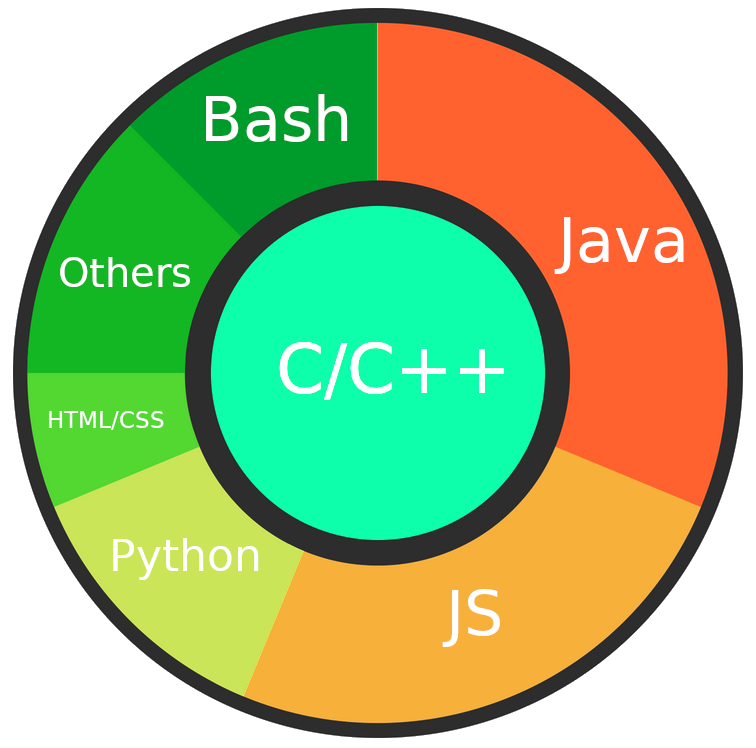
\includegraphics[scale=0.20]{img/programming.png}
    ~
    \section{Personal / Other Skills}
    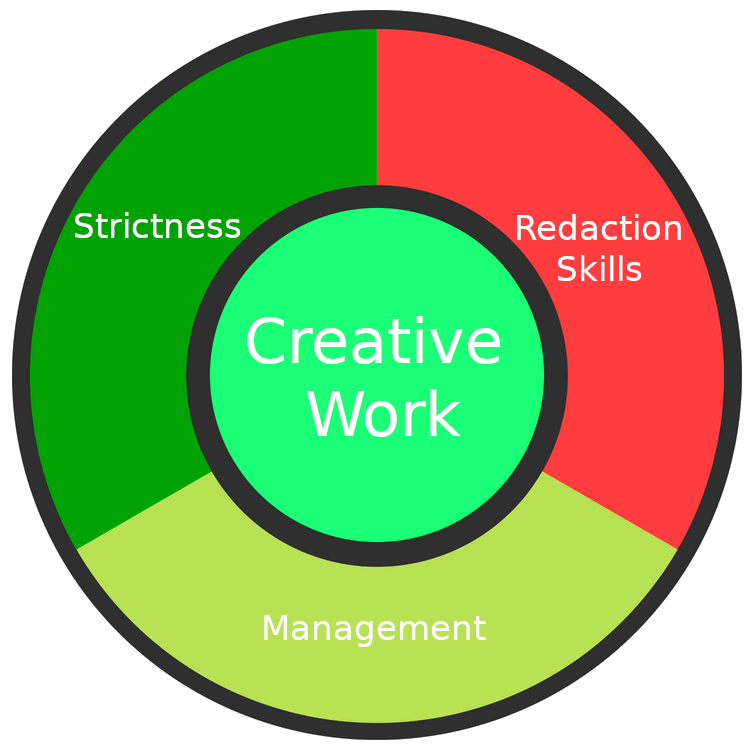
\includegraphics[scale=0.20]{img/personal.png}
    ~
  \section{OS Preference}
    \textbf{GNU/Linux}
\includegraphics[scale=0.40]{img/5stars.png}
    \textbf{Windows}
\includegraphics[scale=0.40]{img/4stars.png}
    \textbf{MacOS}
\includegraphics[scale=0.40]{img/2stars.png}
    ~
    \section{Languages}
    \textbf{Catalan}
\includegraphics[scale=0.40]{img/5stars.png}
    \textbf{Spanish}
\includegraphics[scale=0.40]{img/5stars.png}
    \textbf{English}
\includegraphics[scale=0.40]{img/4stars.png}
    ~
\end{aside}

\section{Experience}
\begin{entrylist}
  \entry
    {09/17 - Now}
    {Part-time collaboration}
    {DEFIB UPC, Barcelona, Spain}
    {Technical maintenance, sysadmin, minor application development, student management.\\}
  \entry
    {03/16 - 03/17}
    {Exhibitor for FIB-UPC}
    {Saló de l'Ensenyament}
    {Exhibitor of my faculty, guide for potential students.\\}
\end{entrylist}

\section{Education}
\begin{entrylist}
  \entry
    {2013 - Now}
    {Bachelor Degree in Informatics Engineering}
    {FIB-UPC, Barcelona, Spain}
    {Finishing studies.\\
    Main subjects: Computer Architecture, HPC related subjects, Embedded Systems.\\
    \emph{Specialization: Computer Engineering.}\\}
  \entry
    {2012 - 2013}
    {Bachelor's Degree in Telecommunications}
    {ETSETB-UPC, Barcelona, Spain}
    {Started the course but changed over to Informatics Engineering the next year.\\}
  \entry
    {2010 - 2012}
    {Scientific Diploma}
    {La Salle, Reus, Spain}
    {Scientific Secondary School.}
\end{entrylist}

\section{Other Courses}
\begin{entrylist}
  \entry
    {06/2017}
    {Architecture and Programming of the GBA}
    {VGA Student Course}
    {\emph{Understanding and Programming of a Low-Level Application for the GBA.}}
  \entry
    {06/2015}
    {Android App Developing}
    {BMA Student Course}
    {\emph{Building an Android App.}}
  \entry
    {07/2011}
    {Image and Graphic Treatment}
    {Centre de la Imatge Mas Iglesias, Reus}
    {\emph{Advanced course about Photoshop treatment for images and graphic design.}}
\end{entrylist}


\section{Other Info and Experience}
Involved in student-driven initiatives like the student delegation (\textit{DEFIB}), the faculty annual party (\textit{FestaFIB}) and the faculty magazine (\textit{l'Oasi}), being part of the directive team and president of the last one for over two years. 

While not being exactly a professional achievement, it has been a fruitful experience on how to manage projects and teams, learning a range of skills related to the creative, administrative and managing processes required for these activities.

You can check all unlisted aptitudes in my LinkedIn.
\\
\begin{flushleft}
\emph{May 15th, 2018}
\end{flushleft}
\begin{flushright}
\emph{Ricard Zarco Badia}
\end{flushright}

\end{document}
